\documentclass{article}
\PassOptionsToPackage{numbers,sort&compress}{natbib}
\usepackage[final,sglblindworkshop]{neurips_2026}
\workshoptitle{Predictive AI Evaluation Competition (PAIEC)}
\usepackage[utf8]{inputenc}
\usepackage[OT1]{fontenc}
\usepackage{amsmath,amsfonts,booktabs}
\usepackage[hidelinks]{hyperref}
\usepackage{url}
\usepackage{graphicx}
\providecommand{\tightlist}{\setlength{\itemsep}{0pt}\setlength{\parskip}{0pt}}
\providecommand{\passthrough}[1]{#1}
\hypersetup{pdftitle={Fixed Shrinkage for Predictive AI Evaluation with Few Observed Labels},pdfauthor={Gioia Zheng}}
\title{Fixed Shrinkage for Predictive AI Evaluation\\with Few Observed Labels}
\author{Gioia Zheng\\TU Darmstadt\\\texttt{gioia.zheng@stud.tu-darmstadt.de}}
\begin{document}
\maketitle
\begin{abstract}
This study compares the acquired-label mean with a fixed Beta(1,1) estimate for predicting model correctness under the PAIEC label budgets. On two exploratory coding benchmarks, mean Brier area under the learning curve decreases from 0.22221 to 0.19527. Fixed-method evaluations on BertaQA and REAL also favor shrinkage in aggregate. On the two coding benchmarks, the one-label budget accounts for about 84\% of the total ALC improvement. Exact acquisition expectations show that variance reduction can offset increased bias, while very low-success groups can suffer. Weaker shrinkage and transferred priors do not satisfy their follow-up criteria. Bounded lexical reweighting improves development ALC, but its average gain on a new TruthfulQA-MC validation is only 0.000037 and reverses under one of three acquisition seeds. It fails the prespecified stability rule. Beta(1,1) remains the submitted method; reliable item-level gains and generalization to hidden benchmarks are not established.
\end{abstract}
\section{Task and research question}\label{task-and-research-question}

The Predictive AI Evaluation Competition evaluates probabilities of binary outcomes without running the target AI system on the test item. Inputs describe the subject, the item, and an anonymous benchmark identifier. A subject is a complete model configuration, including its harness and other evaluation settings. Revealed labels can span several subject-benchmark pairs. The competition uses nested label budgets of 0, 1, 3, 7, 15 and 31, scoring each budget on a fixed evaluation pool \cite{ref1}.

The narrow question here is whether a fixed amount of shrinkage improves probability estimates when very few outcomes are available. An empirical mean based on one binary observation can only predict zero or one. That certainty is often poorly supported. Shrinkage reduces this variation, but introduces bias when the group's success probability is close to an endpoint. Later experiments ask whether cross-benchmark prior transfer or similarity to acquired questions can improve on this estimator. They keep the original candidate as the reference and distinguish development results from subsequently frozen public validations.

\section{Predictors and evaluation}\label{predictors-and-evaluation}

The initial comparison has three predictors sharing the same random acquisition trajectory. Constant 0.5 ignores labels. The official empirical-mean reference \cite{ref2} returns \(s/n\) for \(s\) successes among \(n\) matching labels, and 0.5 when none match. The candidate returns:

\begin{equation}
\widehat p_{\mathrm{Beta}}=(s+1)/(n+2)
\end{equation}

This is the Beta(1,1) posterior-mean formula, used here as a fixed estimator. It adds one pseudo-success and one pseudo-failure, and was fixed before the initial evaluations. The finite-pool analysis below does not require independent identically distributed benchmark items.

A follow-up adds the fixed Beta(0.5,0.5) estimator, \(p=(s+0.5)/(n+1)\). Its strength was chosen after the public development diagnostics and frozen before reading FinanceBench outcomes. It uses the same acquired labels as all three references. There is no parameter grid, fitting, adaptive acquisition or selection using private feedback.

Matching uses all eight visible subject attributes and the anonymous benchmark identifier. Labels from other configurations or benchmarks are ignored. The submitted predictor uses no item text, embeddings, model weights, external data, network calls or persistent state. Its predictions are constant within a subject-benchmark pair at each budget. It estimates group success rates; the later lexical experiment separately tests item-dependent predictions.

For binary response \(y\) and prediction \(p\), Brier loss is \((p-y)^2\). The competition's area under the learning curve (ALC) is the weighted average of Brier scores at the six budgets:

\begin{equation}
\mathrm{ALC}=0.1 B_0+0.2 B_1+0.2 B_3+0.2 B_7+0.2 B_{15}+0.1 B_{31}
\end{equation}

ALC is averaged equally over subject-benchmark pairs. A constant 0.5 prediction gives 0.25 at every budget. Lower values are better \cite{ref1}. Improvements in this proper scoring rule are not, by themselves, evidence that every aspect of calibration improves.

\section{Data and local protocol}\label{data-and-local-protocol}

All experiments use public formatted tables from measurement-db \cite{ref3}, pinned at a fixed revision\footnote{Revision \texttt{54074453da7b9911be0f48e4c560be547bc84d21}.}. The initial exploration uses Multi-SWE-bench \cite{ref5} and ResearchCodeBench \cite{ref6}. BertaQA \cite{ref7} and REAL \cite{ref8} were selected subsequently for non-coding coverage; predictor hashes, seeds and evaluation settings were fixed before their outcomes were inspected. Their results are now observed, so these benchmarks cannot serve as untouched validation data for later changes. All sample counts below refer to these pinned tables, not the original paper releases.

FinanceBench \cite{ref9} supplies the follow-up's new public validation: 150 document-QA items, 16 model/context configurations and 2,400 binary response records. Selection used domain and metadata before its response table was downloaded. The protocol fixes methods, code hashes, seeds, comparisons and decision criteria. All 16 groups meet eligibility, with no missing grades or repeated response cells. No normalized exact matches to the four development benchmarks or within-benchmark lexical duplicates are found. Item and guarded splits yield identical trajectories; this is one validation, not two replications.

Eligible pairs have at least 80 distinct observed items. A fixed split seed, 20261016, determines acquisition and evaluation pools. Acquisition seeds 20261016-20261018 shuffle distinct acquisition items and select one recorded response per revealed item. Label sets are nested. Every recorded response of an evaluation item contributes to the score, using the same probability when inputs are identical. The three seeds share the evaluation pool and are not independent dataset replications.

A guarded split assigns detected related items to the same pool rather than splitting them independently. The coding exploration keeps normalized exact copies and detected lexical near-duplicates together. The lexical check uses token 5-shingle Jaccard similarity at least 0.9, followed by connected components. This design halves cluster counts, so its item fractions can depart from 50/50. An item-ID split provides a sensitivity check closer to the competition's split unit. Both designs keep repeated response runs of an item together.

BertaQA requires a different audit. Its 51,760 prompt variants refer to 4,756 parallel source questions, with English and Basque raw IDs. A label-blind schema inspection led to a source-question sensitivity split that groups translations and prompt variants. Additional lexical matches are computed on final user questions, excluding shared few-shot demonstrations. The primary split remains item based. REAL has no detected exact or 0.9-Jaccard lexical duplicates; its item and guarded splits produce identical trajectories and count as one validation.

Reference answers, grading criteria and response traces are excluded from predictor inputs. The baseline and prior variants ignore the allowed task text; only the lexical follow-up uses it. Repeated observations for the same subject and item are retained rather than collapsed into a single outcome; REAL, for example, has 334 such cells, 91 with differing outcomes.

TruthfulQA-MC \cite{ref10} provides the lexical follow-up's new validation at the same data revision: 817 questions, 150 model configurations and 122,550 binary response records from the preserved Open LLM Leaderboard v1 panel. All groups are eligible, with complete labels and no repeated subject-item cells. Benchmark choice used metadata; the method, seeds and decision rule were fixed before its outcome table was downloaded. Label-blind audits found no within-benchmark or cross-benchmark matches under the stated lexical checks. Its item and guarded trajectories are identical and count as one validation. Shared questions and related model configurations do not constitute 150 independent benchmark replications.

\section{Results and failure analysis}\label{results-and-failure-analysis}

Table \ref{tab:results} reports Brier ALC, averaged equally over eligible pairs and then over the three acquisition seeds. The coding rows use the guarded split; BertaQA and REAL use their fixed primary item splits. Constant 0.5 scores 0.25000 in every row.

\begin{table}[ht]
\centering
\caption{Local Brier ALC, lower is better. Three acquisition seeds share fixed pools. Constant 0.5 has ALC 0.25000 in every row.}
\label{tab:results}
\begin{tabular}{lrrr}
\toprule
Benchmark & Pairs & Empirical mean & Fixed Beta(1,1) \\
\midrule
Multi-SWE-bench & 82 & 0.20334 & 0.18215 \\
ResearchCodeBench & 31 & 0.27213 & 0.22999 \\
BertaQA & 6 & 0.26291 & 0.22409 \\
REAL & 26 & 0.24595 & 0.21036 \\
\bottomrule
\end{tabular}
\end{table}

The initial coding comparison improves from 0.22221 to 0.19527 across 113 pairs. About 84\% of the net improvement comes from budget 1. At budget 31 the aggregate difference is only 0.00021. After averaging seeds, 81 pairs improve and 32 worsen. The coding item split also favors shrinkage, with ALC decreasing from 0.21789 to 0.19367. Because both the pools and the revealed labels change, the difference between split designs does not isolate the effect of duplicate removal.

BertaQA's six configurations all improve after averaging seeds in both its primary and source-question designs. The latter gives 0.27178 for the mean and 0.22645 for shrinkage. About 80\% of the primary split's net improvement comes from budget 1, while shrinkage is slightly worse at budgets 7 and 15. The source-question split eliminates the audited source-group overlap, which affects 2,316-2,433 groups per subject in the item split. These predictors ignore question content, so this sensitivity analysis does not measure the leakage behavior of a retrieval or text-based predictor.

REAL contains 33 subject configurations; seven fail the 80-item eligibility threshold. Its 26 eligible groups contain 89-233 items. Twenty-two improve and four worsen after averaging the three seeds. About 82\% of the sampled net improvement comes from budget 1.

\subsection{Separating acquisition variance from bias}\label{separating-acquisition-variance-from-bias}

The recorded seeds give an incomplete picture of individual groups. Because these predictors are constant within a pair, their expected Brier score can also be calculated exactly over the specified random acquisition policy, conditional on the saved pools.

Let the acquisition pool contain \(N\) items. For item \(i\), let \(\mu_i\) be the proportion of its recorded outcomes equal to one. Define \(m=N^{-1}\sum_i\mu_i\), \(v=N^{-1}\sum_i(\mu_i-m)^2\) and \(u=N^{-1}\sum_i\mu_i(1-\mu_i)\). For a uniform sample of \(n\) distinct items, with one independently selected recorded outcome per item, the success count \(S\) satisfies:

\begin{equation}
\mathbb{E}[S]=n m,\qquad\operatorname{Var}(S)=n\left[\frac{N-n}{N-1}v+u\right],\quad N>1
\end{equation}

When \(N=1\), the between-item term is zero. The first term accounts for sampling items without replacement; the second retains variation among response runs. For a fixed evaluation response success fraction \(q\):

\begin{equation}
\mathbb{E}[\mathrm{Brier}]=\operatorname{Var}(p)+(\mathbb{E}[p]-q)^2+q(1-q)
\end{equation}

The weighted sum gives expected ALC even though budgets are nested, by linearity of expectation. This is retrospective analysis using local outcomes, not information available to the predictor. It averages over acquisition only, not alternative pool splits or future benchmark responses.

The starting kit packs complete groups under a 1,000-source-item cap \cite{ref4}. Restricting the coding exploration to its 85 groups with 80-1,000 items preserves the expected gain (Table \ref{tab:expected}):

\begin{table}[ht]
\centering
\caption{Exact acquisition expectations conditional on fixed pools. Coding includes the 85 groups with 80--1,000 items; REAL includes all 26 eligible groups.}
\label{tab:expected}
\begin{tabular}{lrrrr}
\toprule
Population & \shortstack{Empirical-mean\\ALC} & Beta ALC & Improved & Worsened \\
\midrule
Coding, guarded & 0.26075 & 0.22243 & 73 & 12 \\
REAL, item & 0.23569 & 0.20500 & 21 & 5 \\
\bottomrule
\end{tabular}
\end{table}

On these same 85 coding groups, the observed three-seed ALC is 0.25527 for the empirical mean and 0.21963 for Beta(1,1); all three seeds favor shrinkage. This is a size-compatibility check, not a replay of the hosted draw.

All 12 coding losses occur below 10\% evaluation success. In that retrospective slice, 12 of 14 groups worsen, with mean ALC delta +0.01146. Shrinkage toward 0.5 overestimates these difficult groups. The slice is descriptive; evaluation success cannot be used to choose the prior at prediction time.

At budget 1 in the size-compatible guarded coding subset, a variance reduction of 0.17094 outweighs a squared-bias increase of 0.02293, yielding expected Brier delta -0.14800. Across all 113 coding groups, 15 change their win/loss direction between the three sampled trajectories and exact expectations. The post-review analysis locates all 15 reversals below 20\% evaluation success, including 11 below 10\% (Appendix~\ref{app:postreview}). Aggregate gains are more stable than conclusions about every individual group.

\subsection{Weaker shrinkage: a negative aggregate result}\label{weaker-shrinkage-a-negative-aggregate-result}

The follow-up asks whether weaker fixed shrinkage reduces low-success bias while retaining the benefit of a few labels. An overall advantage requires lower observed and exact expected ALC than Beta(1,1) on FinanceBench, observed ALC below the empirical mean, a mean Brier advantage over the empirical mean at budgets 1 and 3, and no reversal under the guarded split. The four previously inspected benchmarks are development reanalyses, not additional prospective validations.

\begin{table}[ht]
\centering
\caption{Weaker-prior ablation. Observed Brier ALC for Beta($\alpha,\alpha$); difference is weaker minus baseline. Each row averages the same three acquisition seeds.}
\label{tab:weaker}
\small
\begin{tabular}{llrrr}
\toprule
Benchmark & Role & $\alpha=1$ & $\alpha=0.5$ & Difference \\
\midrule
Multi-SWE-bench & Development & 0.182148 & 0.182152 & +0.000005 \\
ResearchCodeBench & Development & 0.229991 & 0.236628 & +0.006637 \\
BertaQA & Development & 0.226454 & 0.234033 & +0.007579 \\
REAL & Development & 0.210362 & 0.214798 & +0.004435 \\
FinanceBench & New validation & 0.202287 & 0.205503 & +0.003215 \\
\bottomrule
\end{tabular}
\end{table}

Table \ref{tab:weaker} uses guarded coding pools, BertaQA source-question pools, and item pools for REAL and FinanceBench. In particular, the BertaQA row differs from the primary item split above. All rows include every locally eligible group; the larger BertaQA and coding groups need not fit the hosted draw cap.

On FinanceBench, weaker shrinkage improves six groups and worsens ten after averaging seeds. The aggregate direction is adverse under all three seeds. Exact expected ALC also increases, from 0.195384 to 0.197041. The weaker estimator still beats the empirical mean's observed ALC of 0.234080 and retains its small-budget advantage, but the prespecified overall criterion fails. A post-review pair bootstrap gives a 95\% interval of [-0.00141, +0.00801] for its difference from Beta(1,1); the result does not establish that weaker shrinkage is significantly worse. Beta(1,1) remains the candidate; no strength is adjusted after this result.

The two groups with evaluation success below 10\% improve: their observed ALC falls from 0.113542 to 0.104443, and expected ALC from 0.107401 to 0.096816. However, the empirical mean's expected ALC in this slice is lower still, at 0.094770. This slice was specified before evaluation but uses evaluation labels to determine membership, so it is diagnostic rather than a prediction-time choice rule.

Across all FinanceBench groups at budget 1, weaker shrinkage reduces squared bias by 0.016975 but increases prediction variance by 0.023299. Expected Brier therefore rises by 0.006324: reduced bias does not offset the lost variance reduction.

\section{Extensions beyond fixed shrinkage}\label{extensions-beyond-fixed-shrinkage}

\subsection{Transferring a prior across benchmarks}\label{transferring-a-prior-across-benchmarks}

The five previously inspected benchmarks form a development set for this round. In each leave-one-benchmark-out fold, a transferred center \(\mu\) is the equal average of the other four benchmark means, each itself an equal average of eligible subject-group success rates. All outcomes from the target benchmark are excluded from fitting. The predictor is \((s+2\mu)/(n+2)\), retaining prior strength two. This tests transfer across benchmarks, not unseen models.

An adaptive variant starts with equal weights on Beta(1,1) and Beta(\(2\mu,2(1-\mu)\)), then updates the weights using the marginal likelihood of the matching acquired labels. A fixed 50/50 mixture is an ablation. Evaluation reuses the saved pools and seeds. Exact finite-pool expectations for the nonlinear mixture use the success-count distribution; exhaustive small examples check this calculation.

\begin{table}[ht]
\centering
\caption{Prior-transfer development results on five previously inspected benchmarks. All methods share item splits and acquisition trajectories. Lower Brier ALC is better.}
\label{tab:transfer}
\begin{tabular}{lrr}
\toprule
Method & Equal-pair ALC & Equal-benchmark ALC \\
\midrule
Beta(1,1) & 0.198355 & 0.209376 \\
Transferred center & 0.196179 & 0.211976 \\
Fixed mixture & 0.197093 & 0.210236 \\
Adaptive mixture & 0.197112 & 0.210257 \\
\bottomrule
\end{tabular}
\end{table}

The competition-style equal-pair average improves, but both transferred variants worsen the equal-benchmark average used as a robustness check. They fail the development criteria, including the exact-expectation comparisons, and do not proceed to new validation. BertaQA exposes the mismatch: transferring a center near 0.347 raises ALC from 0.224091 to 0.250606. The adaptive mixture reduces this to 0.235935 but still loses to the baseline. At zero labels there is no evidence to reject a mismatched prior. More generally, favoring larger benchmark panels can obscure a substantial loss on a smaller panel. Equal-benchmark averaging is an additional diagnostic, not the official scoring rule.

\clearpage
\subsection{Bounded lexical reweighting}\label{bounded-lexical-reweighting}

The lexical variant fits TF-IDF only on the current matching acquired questions. It uses Unicode-normalized word tokens, logarithmic term frequency and smoothed inverse document frequency. Let \(c_i\) be the cosine similarity between the target and acquired item \(i\). For \(n\) labels, the weights and prediction are

\begin{equation}
w_i=\frac{n(1+c_i)}{n+\sum_j c_j},\qquad
\widehat p_{\rm lex}=\frac{1+\sum_i w_i y_i}{n+2}.
\end{equation}

The weights sum to \(n\), their ratio is at most two, and predictions at zero or one label equal the baseline. Empty text and uniform similarity also recover the baseline. No parameters are selected using evaluation outcomes. For serialized chat lists, features use only the final user message; other content remains intact. This excludes BertaQA demonstrations. TruthfulQA uses serialized prompt objects, so its shared few-shot examples remain in the features. This limitation was recorded before its outcomes were read.

\begin{table}[ht]
\centering
\caption{Lexical reweighting versus the baseline and a shuffled-label control. The guarded development design reuses REAL and FinanceBench once. TruthfulQA item and guarded trajectories coincide.}
\label{tab:retrieval}
\small
\begin{tabular}{lrrrr}
\toprule
Population & Groups & Beta(1,1) & Lexical & Shuffled \\
\midrule
Development, item & 161 & 0.198355 & 0.198029 & 0.198412 \\
Development, guarded & 161 & 0.199569 & 0.199339 & 0.199592 \\
TruthfulQA, new validation & 150 & 0.227169 & 0.227132 & 0.227166 \\
\bottomrule
\end{tabular}
\end{table}

The control keeps similarity weights fixed and deterministically permutes the acquired labels within each group, seed and budget. It uses one permutation per case and is a diagnostic, not a significance test. The development item design improves 121 groups, worsens 36 and ties four. Equal-benchmark ALC falls from 0.209376 to 0.209015; the guarded average falls from 0.210248 to 0.210000. BertaQA slightly worsens in both designs. Guarding uses the coding near-duplicate and BertaQA source-question splits; REAL and FinanceBench are reused once because their designs coincide. All five datasets remain development evidence.

The frozen TruthfulQA rule requires lower mean ALC under both split designs, lower ALC for each of the three acquisition seeds, and an advantage over the shuffled-label control. The mean improves by 0.000036893, with 85 groups improving and 65 worsening. The three seed deltas, lexical minus baseline, are \(+0.000034541\), \(-0.000039481\) and \(-0.000105740\). Thus the stability rule fails, although the average beats both controls. It is a conservative selection rule, not a statistical test or proof that the method cannot help. No changes to the extractor, weights or benchmark choice follow this result. Beta(1,1) remains the candidate.

\section{Implementation and reproducibility}\label{implementation-and-reproducibility}

Code for the original experiments is available at \href{https://github.com/GioiaZheng/paiec-2026/tree/d2d3e3c1e803880f4918f2f8065616b513731a40}{GioiaZheng/paiec-2026}, revision \texttt{d2d3e3c}, under MIT. The release includes the baseline and weaker-prior comparisons, the later extensions, and a clean-workspace reproduction driver with pinned inputs and aggregate references.

The empirical-mean and Beta(1,1) archives pass the kit's ZIP and smoke checks. The candidate contains \texttt{model.py} and a README, needs only Python's standard library, and has identical Windows and Linux hashes. The supplementary archive preserves both original files byte for byte and passes the official ZIP check.

Replay with four official workers covers six groups and three benchmarks. Probabilities and pairwise Brier/ALC agree within \(10^{-12}\). This checks packaging and workers, not private sampling; Appendix A records the verification workload.

Experiments use Python 3.12.2 and PyArrow 23.0.1 on Windows; Ubuntu WSL replay uses Python 3.14.4. No GPU or paid API is used. Configurations, hashes, commands and aggregates accompany the code. Independent recomputation checks the weaker-prior comparison, whose module passes the kit's sequential smoke check.

All 19 original project tests pass, covering exhaustive acquisition expectations, hand-calculated lexical weights and group isolation. Independent rescoring checks the lexical predictions against response rows. The lexical ZIP passes official local checks and four-worker Linux replay. No extension is uploaded to CodaBench.

A clean workspace rebuilds eight split runs directly from the 24 pinned tables, without the original saved runs. All four follow-up aggregate summaries and selection decisions match within absolute tolerance \(10^{-12}\). This verifies numerical reproducibility; it supplies no new validation evidence. Appendix B gives the entry point.

\subsection{Official formative feedback}\label{official-formative-feedback}

Submission 992850 completed on 16 October 2026 with Brier ALC 0.165110. Feedback covers eight subject-benchmark combinations, seven anonymous benchmarks and 497 unique evaluation subject-item pairs. Macro Brier falls from 0.250000 at budget zero to 0.138299 at budget 31. Seven combinations have lower ALC than constant 0.5; one has higher ALC.

This formative score agrees with the displayed budget curves within 0.000001. It is not a final result or a paired comparison against empirical mean. Raw execution output is hidden. Private feedback remains local and does not enter model fitting.

\section{Limitations}\label{limitations}

Six public benchmarks offer limited generalization evidence. Appendix~\ref{app:postreview} adds post-review paired bootstrap and calibration diagnostics using already observed data. Their intervals describe resampling of this small, dependent panel; they do not establish coverage for future benchmarks or a final competition result. The later hypotheses were informed by previous results; only the subsequent frozen comparisons on newly selected benchmarks provide prospective public evidence. The conservative seed rule cannot establish statistical significance. FinanceBench and TruthfulQA are now observed data for any future changes.

Local group coverage also differs from the hosted draw. Each BertaQA subject has 9,512 observed items and cannot fit as a complete group under the kit's 1,000-item cap. Its results describe a broader local population. The kit skips complete groups that exceed the remaining cap; truncating BertaQA to sampled subgroups would change that contract. Filtering coding groups by size and choosing small REAL groups addresses this mismatch only partly: neither reproduces the organizer's balancing and random group selection.

Lexical and source-ID audits do not rule out semantic duplication or shared-document effects. Model identities may recur across benchmarks; this is not an unseen-model evaluation. The submitted estimator cannot discriminate item difficulty. Lexical gains shrink on the new benchmark and vary with acquisition seed; the results do not isolate whether domain, shared prompt material or sampling causes this change. Exact acquisition expectations concern stored responses and apply to the group-rate predictors, not the item-dependent lexical method.

\section*{Development disclosure}\label{development-disclosure}

OpenAI Codex assisted with implementation, verification scripts, analysis and drafting. No language model or external API is called by the candidate predictor.

\label{main-end}
\clearpage
\begin{thebibliography}{10}
\bibitem{ref1}
Stanford AIMS. \href{https://aims.stanford.edu/competition}{Predictive AI Evaluation Competition}. Rules accessed 31 October 2026.
\bibitem{ref2}
AIMS Foundations. \href{https://github.com/aims-foundations/paiec_baseline/tree/cc88a959c1e5e7462f31a9215baba066ce6d6e2b}{PAIEC reference baselines}. Pinned source revision; MIT license.
\bibitem{ref3}
AIMS Foundations. \href{https://huggingface.co/datasets/aims-foundations/measurement-db/tree/54074453da7b9911be0f48e4c560be547bc84d21}{measurement-db}. Public formatted tables for the six benchmarks in this report; source data are not redistributed.
\bibitem{ref4}
PAIEC organizers. \href{https://www.codabench.org/datasets/download/4ae12cd5-cc62-4c11-bad5-d9a51381b39b/}{CodaBench starting kit}. Sampling and runtime documentation; archive hash recorded in the reproduction evidence.
\bibitem{ref5}
Daoguang Zan et al.~\href{https://arxiv.org/abs/2504.02605}{Multi-SWE-bench: A Multilingual Benchmark for Issue Resolving}. arXiv:2504.02605, 2025.
\bibitem{ref6}
Tianyu Hua et al.~\href{https://arxiv.org/abs/2506.02314}{ResearchCodeBench: Benchmarking LLMs on Implementing Novel Machine Learning Research Code}. arXiv:2506.02314, 2025.
\bibitem{ref7}
Julen Etxaniz, Gorka Azkune, Aitor Soroa, Oier Lopez de Lacalle and Mikel Artetxe. \href{https://arxiv.org/abs/2406.07302}{BertaQA: How Much Do Language Models Know About Local Culture?}. arXiv:2406.07302, 2024.
\bibitem{ref8}
Divyansh Garg et al.~\href{https://arxiv.org/abs/2504.11543}{REAL: Benchmarking Autonomous Agents on Deterministic Simulations of Real Websites}. arXiv:2504.11543, 2025.
\bibitem{ref9}
Pranab Islam et al.~\href{https://arxiv.org/abs/2311.11944v1}{FinanceBench: A New Benchmark for Financial Question Answering}. arXiv:2311.11944, 2023.
\bibitem{ref10}
Stephanie Lin, Jacob Hilton and Owain Evans. \href{https://aclanthology.org/2022.acl-long.229/}{TruthfulQA: Measuring How Models Mimic Human Falsehoods}. Proceedings of ACL, pages 3214-3252, 2022.
\end{thebibliography}
\clearpage
\appendix
\section{Reproduction outline}
The commands below refer to the submitted checkout \texttt{d2d3e3c}, whose
scripts live at the root, not the later \texttt{experiments/} directory.
Create a separate checkout:
\begin{verbatim}
git clone --config core.autocrlf=false \
  https://github.com/GioiaZheng/paiec-2026.git submitted-code
git -C submitted-code checkout \
  d2d3e3c1e803880f4918f2f8065616b513731a40
cd submitted-code
\end{verbatim}
Use Python 3.12 and the pinned reference baseline. Obtain the four formatted
tables per benchmark through authorized measurement-db access at the revision
in Section 3 and place them in \texttt{data/<benchmark>/}. Manifests record
their hashes. Source tables are not redistributed; ResearchCodeBench, REAL
and FinanceBench have unknown license metadata.

\paragraph{Build and check.}
Unpack the competition starting kit under \texttt{local/official/starting\_kit}.
From the submitted checkout root:
\begin{verbatim}
python -m pip install --target .deps -r requirements-local.txt
python run_baseline.py --starter-kit local/official/starting_kit
python -m unittest test_evaluation.py test_diagnostics.py
python -m unittest test_weaker_shrinkage.py
\end{verbatim}

\paragraph{Run and verify.}
The default pilot is coding with the guarded split. Set \texttt{--protocol}
and \texttt{--split-unit} as follows for the other designs:
\begin{center}
\begin{tabular}{lll}
\toprule
Dataset & Protocol file & Split options \\
\midrule
Coding & None (default) & \texttt{near}, \texttt{item} \\
BertaQA & \path{configs/bertaqa-validation.json} & \texttt{item}, \texttt{source} \\
REAL & \path{configs/real-validation.json} & \texttt{item}, \texttt{near} \\
FinanceBench & \path{configs/weaker-shrinkage.json} & \texttt{item}, \texttt{near} \\
\bottomrule
\end{tabular}
\end{center}
\begin{verbatim}
python evaluate_pilot.py
python verify_pilot.py runs/<run-id>
python analyze_pilot.py runs/<run-id>
python compare_shrinkage.py runs/<verified-run>
\end{verbatim}
Each pilot prints its new run directory. The verifier recomputes response-level
scores and pool separation. Pass verified coding-guarded, BertaQA-source,
REAL-item and FinanceBench runs together to \texttt{compare\_shrinkage.py}
to reproduce the ablation. It checks source hashes and saved labels;
\texttt{diagnose\_shrinkage.py} supplies the original expectation analysis.
Neither fits a predictor. Replay commands for four Linux workers and input
setup are in the submitted checkout's \texttt{REPRODUCIBILITY.md}.

\paragraph{Executed verification.}
Baseline replay covers 962 source subject-item pairs and 760 response rows,
with 473 calls and 287 reused predictions per checkpoint. The weaker-prior
check covers 11,592 probability/budget records across 161 groups. Lexical
rescoring covers 4,439,754 item-budget-seed records, including identical split
designs; Linux replay checks 4,560 response-level predictions. These are
verification workloads, not independent statistical sample sizes. Private
item-level outcomes and anonymous group identities are excluded from the report.
\clearpage
\section{Follow-up specification and local evidence}
\paragraph{Prior transfer and mixture.}
In each fold, average the full-response success rates of eligible groups within
each source benchmark, then average those source-benchmark means equally.
Exclude the complete target benchmark. Both prior strengths remain two.
For component $k$ with parameters $(a_k,b_k)$ and $s$ successes in $n$ labels,
the adaptive weight is proportional to
$\tfrac12 B(a_k+s,b_k+n-s)/B(a_k,b_k)$, normalized over the two components.
The prediction is the weighted sum of $(s+a_k)/(n+a_k+b_k)$.
The static ablation keeps weights at $1/2$.

\paragraph{Lexical features.}
Normalize text with Unicode NFKC and case folding, then extract word tokens.
Term frequency is $1+\log c_t$ for nonzero count $c_t$.
On the $n$ revealed matching texts, use
$\mathrm{idf}_t=1+\log[(n+1)/(\mathrm{df}_t+1)]$; unseen target terms have
$\mathrm{df}_t=0$. Normalize TF-IDF vectors to unit length for cosine similarity.
Only the acquired prefix determines IDF. No evaluation labels or target-corpus
frequencies enter fitting. A target with no tokens has zero similarity to all
acquired items. The baseline is returned directly for zero or one matching label.
The control shuffles only labels, preserving the text-derived weights and success count.

\paragraph{Frozen sequence.}
All five earlier benchmarks are development data for prior transfer, adaptive
mixing and lexical screening. TruthfulQA selection and the full lexical protocol
were frozen before its outcome table was downloaded on 31 October. Source,
metadata and outcome-file hashes are recorded. A zero-label compatibility guard
for the official ZIP fixture was added before validation and checked to preserve
valid-input predictions; the development source remains archived separately.

\paragraph{Evidence and release scope.}
The reviewed release at \texttt{d2d3e3c} includes the baseline and follow-up
source, configurations, aggregate reference and reproduction guide. The
supplementary archive contains the same 66 code files and the unchanged
candidate. The build manifest records the evidence for Tables~\ref{tab:transfer}
and~\ref{tab:retrieval}, the successful clean replication, and verification
of the published code.

\paragraph{Clean replication.}
After installing the pinned dependency and obtaining the upstream baseline and
six benchmarks, run from the project root:
\begin{verbatim}
python -X utf8 reproduce_extensions.py --output local/replication
\end{verbatim}
The destination must not exist. The driver checks all data and source hashes,
normalizes source line endings, rebuilds eight split runs, and recomputes all
follow-ups. It independently rescores the lexical predictions and compares all
aggregate summaries and selection flags with the recorded reference, to absolute
tolerance $10^{-12}$. The experiment subprocesses use the copied code and installed
dependency. No old run outputs or network access are used. The input snapshots are explicitly
marked as replication records, not a new prospective freeze. Commands and input
paths are in \path{docs/extensions-reproduction.md}; a successful run writes
\path{replication.json} in its output directory.

Raw tables and prediction traces stay local. TruthfulQA questions are Apache-2.0;
the preserved leaderboard observations have no separate declared data license
in the captured metadata and are not redistributed.

\clearpage
\section{Post-review diagnostics}\label{app:postreview}
These analyses were specified and run on 21 November 2026 in response to
review, after all reported outcomes had been inspected. They reuse the
saved pools and acquisition trajectories, do not select a predictor, and
provide no new held-out validation. The submitted estimator and numerical
results in original Tables~\ref{tab:results}--\ref{tab:retrieval} are unchanged.

\subsection{Paired uncertainty summaries}
For each method comparison, first average its paired ALC differences over
the three acquisition seeds within each subject-benchmark pair. Resample
these pair-level differences with replacement separately within each benchmark,
preserving its pair count. We use 20,000 draws, random seed 20261121, and the
2.5th and 97.5th percentiles with linear interpolation. Table~\ref{tab:intervals}
reports the differences and descriptive 95\% bootstrap intervals. No seed or
response row is treated as an independent population replicate.

\begin{table}[ht]
\centering\small
\caption{Post-review paired ALC intervals. Negative favors the first method.
Split designs match their respective original tables; BertaQA uses item
pools in the first panel and source-question pools in the second.}
\label{tab:intervals}
\begin{tabular}{lrrl}
\toprule
Benchmark & Pairs & Difference & Pair bootstrap interval \\
\midrule
\multicolumn{4}{l}{Beta(1,1) minus empirical mean (Table~\ref{tab:results})} \\
Multi-SWE-bench & 82 & -0.021193 & [-0.02804, -0.01413] \\
ResearchCodeBench & 31 & -0.042135 & [-0.05216, -0.03140] \\
BertaQA & 6 & -0.038817 & [-0.05639, -0.02275] \\
REAL & 26 & -0.035584 & [-0.04682, -0.02308] \\
\midrule
\multicolumn{4}{l}{Beta(0.5,0.5) minus Beta(1,1) (Table~\ref{tab:weaker})} \\
Multi-SWE-bench & 82 & +0.000005 & [-0.00207, +0.00207] \\
ResearchCodeBench & 31 & +0.006637 & [+0.00339, +0.00968] \\
BertaQA & 6 & +0.007579 & [+0.00474, +0.01067] \\
REAL & 26 & +0.004435 & [+0.00059, +0.00787] \\
FinanceBench & 16 & +0.003215 & [-0.00141, +0.00801] \\
\bottomrule
\end{tabular}
\end{table}

The primary comparison across 145 pairs has mean difference -0.02898
and a stratified-pair interval \mbox{[-0.03401, -0.02382]}. Across the 161 pairs in the weaker-prior
comparison, the mean difference is +0.00260, with interval \mbox{[+0.00116, +0.00403]}.
The latter averages development and validation panels and is not a new
confirmatory test. The FinanceBench-only interval crosses zero: failing
the original replacement rule is distinct from proving inferiority.

As a dependence sensitivity check, resample whole benchmark panels instead,
retaining all their pairs and recomputing the equal-pair mean for every draw.
The corresponding intervals are \mbox{[-0.04160, -0.02239]} (four primary benchmarks)
and \mbox{[+0.00058, +0.00621]} (five weaker-prior benchmarks). These are conditional
resampling summaries, not reliable population-coverage statements: questions
and related model configurations are shared within panels, model identities can
recur between panels, and four or five benchmarks provide little information
about between-benchmark variation. Neither procedure averages over new pool
splits, unobserved responses or acquisition trajectories beyond the three saved
seeds. The exact expectations in Section~4 average acquisition more fully,
but are likewise conditional on the saved pools.

\clearpage
\subsection{Population sensitivity and individual reversals}
The 85 coding groups with 80--1,000 source items have observed ALC 0.25527
(empirical mean) versus 0.21963 (Beta(1,1)), compared with exact expectations
0.26075 and 0.22243. Per-seed observed differences are -0.03816, -0.03791, -0.03086.
These groups fit individually under the kit cap. Joint inclusion still depends
on benchmark/subject balancing, random tie-breaking and the remaining budget;
the figures do not reproduce that selection. The kit admits complete groups
and skips those that do not fit. In particular, the six 9,512-item BertaQA
groups would be excluded under this contract, not randomly truncated.
We therefore do not describe a BertaQA subgroup experiment as hosted-like.

To examine composition sensitivity, let $f$ be an imposed fraction of groups
with evaluation success below 10\%. Holding equal weights within each of the
two observed strata, the reweighted difference is
\begin{equation}
\Delta(f)=f\,\overline\Delta_{q<0.1}+(1-f)\,\overline\Delta_{q\geq0.1}.
\end{equation}
This uses evaluation outcomes retrospectively and supplies no feasible
test-time selection rule. It changes the group mix, not individual predictions.

\begin{table}[ht]
\centering\small
\caption{Coding sensitivity to the imposed low-success share $f$.
Differences are Beta(1,1) minus empirical mean; positive favors the mean.}
\label{tab:reweight}
\begin{tabular}{rrrrr}
\toprule
& \multicolumn{2}{c}{All 113 coding groups} & \multicolumn{2}{c}{85 size-compatible groups} \\
$f$ & Observed & Expected & Observed & Expected \\
\midrule
0.00 & -0.04381 & -0.04487 & -0.04627 & -0.04813 \\
0.25 & -0.03057 & -0.03037 & -0.03014 & -0.03323 \\
0.50 & -0.01733 & -0.01587 & -0.01402 & -0.01834 \\
0.75 & -0.00409 & -0.00136 & +0.00210 & -0.00344 \\
1.00 & +0.00915 & +0.01314 & +0.01823 & +0.01146 \\
\bottomrule
\end{tabular}
\end{table}

The original low-success shares are 36/113 (31.9\%) and 14/85 (16.5\%).
For all coding groups, the expected difference crosses zero at $f=0.773$;
the observed-seed difference crosses at $f=0.827$. For the size-compatible
subset the corresponding crossings are 0.808 and 0.717. These are algebraic
break-even points for fixed observed stratum means, not estimated universal
thresholds. The change between populations and between sampled and expected
scores shows why a mean improvement need not persist under a harder group mix.

All 15 coding sign reversals lie between 0.99\% and 19.68\% evaluation
success: 11 below 10\%, four in [10\%, 20\%), and none at or above 20\%.
Nine show an observed gain but an expected loss; six show an observed loss
but an expected gain. They are concentrated among low-success groups rather
than spread across the success-rate range. The lowest rate is about 1\%, so
this is not evidence of a sharp boundary specifically at 10\%.

\clearpage
\subsection{Calibration at the smallest nonzero budgets}
At budgets 1 and 3, each predictor takes only two or four distinct values,
respectively. We group by these exact probabilities rather than choosing
histogram bins. Every subject-benchmark pair and acquisition seed receives
equal weight; within a pair-seed case, evaluation response rows share its
weight equally. Thus repeated runs retain their scoring role without allowing
large pools to dominate the equal-pair objective. For category $j$, let $w_j$
be its weight, $p_j$ its prediction, and $\bar y_j$ its weighted outcome rate.
With overall rate $\bar y$, the weighted decomposition is
\begin{equation}
\mathrm{Brier}=
\underbrace{\sum_j w_j(p_j-\bar y_j)^2}_{\mathrm{reliability}}
-\underbrace{\sum_j w_j(\bar y_j-\bar y)^2}_{\mathrm{resolution}}
+\underbrace{\bar y(1-\bar y)}_{\mathrm{uncertainty}}.
\end{equation}
Direct response-level scoring and this identity agree within $10^{-12}$.
Table~\ref{tab:calibration} uses the 145 pairs and split designs of
Table~\ref{tab:results}. Lower reliability is better; this finite-sample
diagnostic is not a population calibration guarantee.

\begin{table}[ht]
\centering\small
\caption{Exact-category calibration summaries, pooled across the primary four
benchmarks. Resolution and uncertainty are shared by both methods.}
\label{tab:calibration}
\begin{tabular}{rlrrrr}
\toprule
Budget & Method & Brier & Reliability & Resolution & Uncertainty \\
\midrule
1 & Empirical mean & 0.34772 & 0.14772 & 0.00637 & 0.20636 \\
1 & Beta(1,1) & 0.22702 & 0.02702 & 0.00637 & 0.20636 \\
3 & Empirical mean & 0.22415 & 0.03392 & 0.01613 & 0.20636 \\
3 & Beta(1,1) & 0.20330 & 0.01307 & 0.01613 & 0.20636 \\
\bottomrule
\end{tabular}
\end{table}

\begin{figure}[ht]
\centering
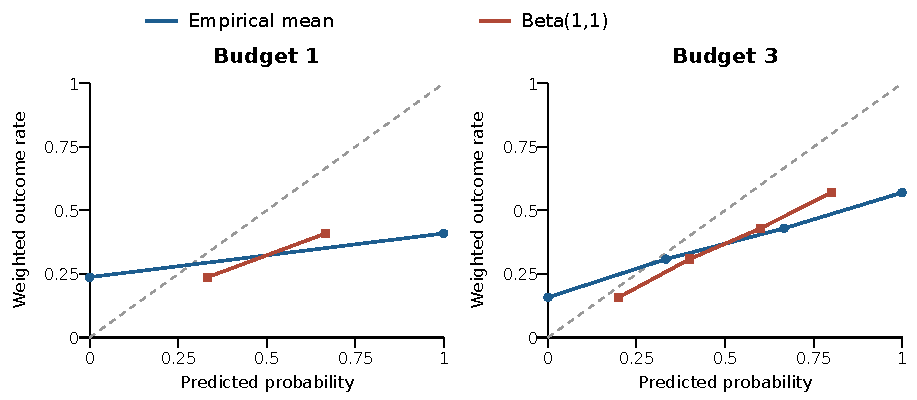
\includegraphics[width=\linewidth]{figures/reliability.pdf}
\caption{Weighted outcome rate against each exact prediction value. The dashed
line denotes perfect reliability; joining points is a visual guide only.
The same outcome groups move horizontally when shrinkage is applied.}
\label{fig:reliability}
\end{figure}

Reliability decreases at both budgets in each of the four benchmarks
separately as well as in the pooled panel. Shrinkage is an injective affine
transform of the success count at a fixed budget, so it preserves category
membership and resolution exactly. These gains concern less extreme group
probabilities, not newly learned item discrimination. Pooling may conceal
subgroup miscalibration, and no binomial error bars are attached to the shared
evaluation outcomes or repeated seed cases.

\paragraph{Recomputing the additions.}
The \href{https://github.com/GioiaZheng/paiec-2026/releases/download/camera-ready-2026-11-21/paiec-camera-ready-source.zip}{camera-ready diagnostic bundle (fixed release: camera-ready-2026-11-21)}
separates these additions from the original experiments at \texttt{d2d3e3c}.
It contains the configuration, aggregate group inputs, scripts, tests and hashes.
Run \texttt{python analysis/analyze.py} from the extracted bundle using
Python 3.12 to regenerate the statistics. The optional collector checks the
pinned response tables and saved trajectories: 6,012 original probability/budget
records across 167 pair/split combinations agree. No raw item text or response
traces are included. The original code pin and CodaBench submission remain unchanged.

\end{document}
